\documentclass[10pt, a4paper]{article} % 设置字体大小和纸张类型
\usepackage{fontspec}
\setmainfont{Times New Roman}

\usepackage{booktabs} % 支持更专业的表格线条
\usepackage{ctex}
\usepackage{caption} % 插图和表格的标题格式
\usepackage{amsmath, amsfonts, amssymb} % 数学公式支持
\usepackage{graphicx} % 插入图片
\usepackage{hyperref} % 超链接支持
\usepackage{hypcap} % 修正超链接指向的图片位置
\usepackage{geometry}
\usepackage{titlesec}
\usepackage{fmtcount} % 用于数字到中文的转换
\usepackage{enumitem} % 加载 enumitem 宏包
\usepackage{multirow} % 支持多行单元格
\usepackage{diagbox}
\usepackage{makecell} % 支持单元格内换行
\usepackage{tikz}
\usepackage{makecell}
\usepackage{unicode-math}
\setmathfont{Latin Modern Math}



\renewcommand{\thesection}{\chinese{section}、}
\renewcommand{\thesubsection}{\arabic{subsection}.}


\begin{document}

\begin{titlepage}
    \newgeometry{left=0cm, right=0cm, top=0cm, bottom=0cm}
    \centering
    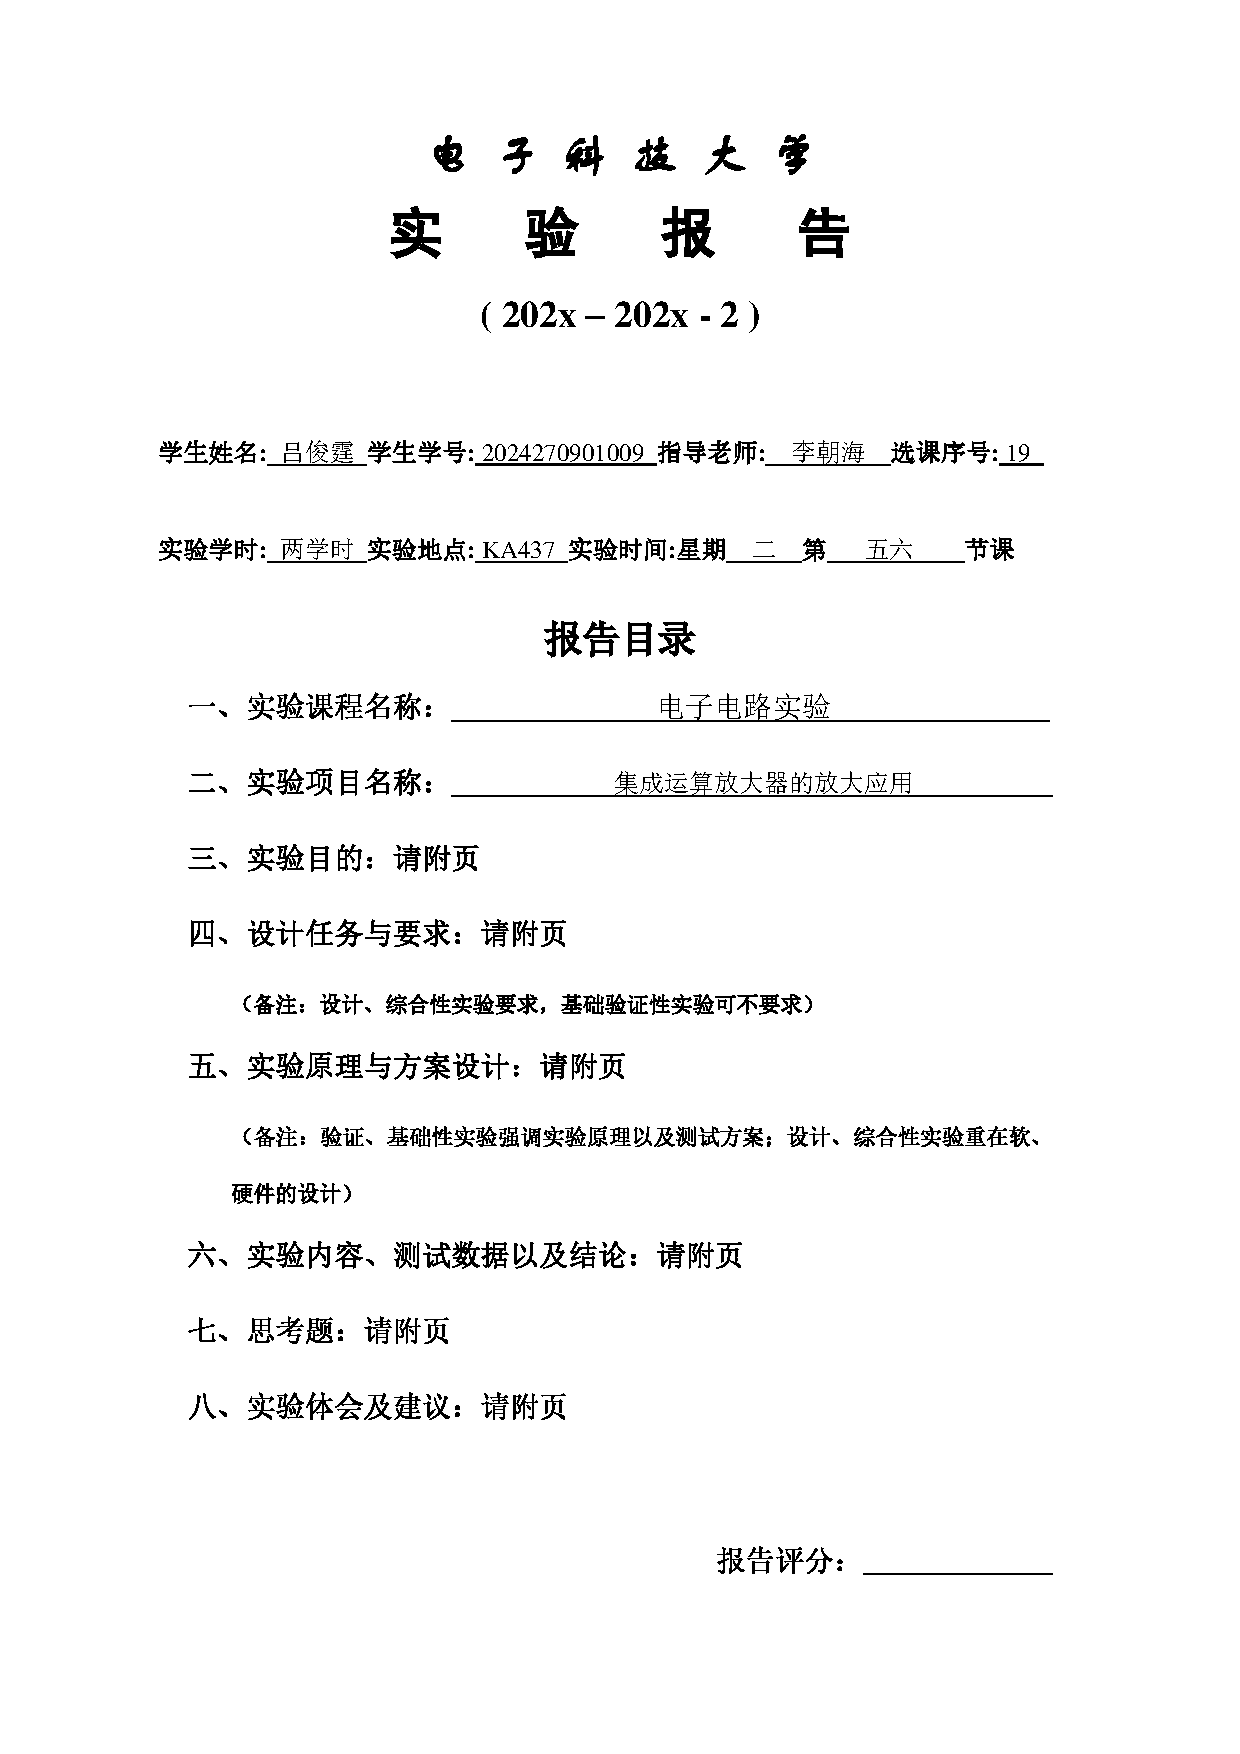
\includegraphics[page=1, width=0.9\textwidth, keepaspectratio]{image/实验报告撰写封面.pdf}
    \restoregeometry
\end{titlepage}

\setcounter{section}{2}

\section{实验目的}

\begin{enumerate}[leftmargin=50pt,label=(\arabic*)] % 设置序号格式为(1)
    \item 了解集成运算放大器的基础知识; 
    \item 学习集成运算放大器的外部特性及使用方法; 
    \item 理解集成运放构成的比例放大器原理。
\end{enumerate}

\section{设计任务与要求}

暂不需要。

\section{实验原理与方案设计}
\subsection{实验原理}
集成电路( IC )按功能可分为模拟集成电路和数字集成电路。模拟集成电路用来产生、放大和处理各类连续变化的模拟量电信号。

集成运算放大器( OP ), 简称运放, 是模拟集成电路中应用最广泛的一种, 实质上是一种集成化的直接耦合式的多级放大器, 具有高增益, 高输入电阻、低输出电阻等特点。可以在负反馈之后对信号进行加减乘除积分微分指数对数等运算。
国际图形符号如图1所示。

\begin{figure}[ht]
    \centering
    \begin{minipage}{0.45\linewidth}
        \centering
        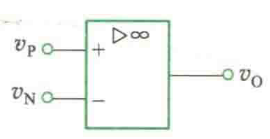
\includegraphics[width=\linewidth]{image/1.png}
        \caption{IEC国际标准符号}
        \label{fig:op_amp_symbol}
    \end{minipage}
    \hfill
    \begin{minipage}{0.45\linewidth}
        \centering
        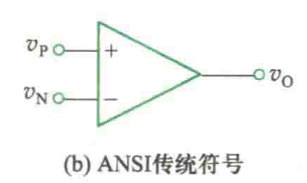
\includegraphics[width=\linewidth]{image/2.png}
        \caption{ANSI传统符号}
    \end{minipage}
\end{figure}




\subsection*{( 1 )集成运算放大器分类}

根据电路结构的不同, 运算放大器可以分为电压反馈放大器( voltage feedback amplifier, VFA )和电流反馈放大器( current feedback amplifier, CFA )两类。本书所指运算放大器为VFA。

虽然运放的内部结构基本相同( 一般由差分输入级、中间放大级、输出级和偏置电路四部分组成 ), 但随着工艺的发展和性能的改善, 逐渐衍生出品种繁多的运算放大器类型。

\subsubsection*{1.按照制造工艺分类}

\begin{enumerate}
    \item[A.] 通用型运放
    
    具有运放最基本的功能, 各项参数比较均衡, 价格低廉, 可满足大多数情况下的使用要求, 如 $\mu A741$、LM358、LM324 等。
    
    \item[B.] 精密型运放
    
    精密型运放对输入失调电压、输入偏置电流、温度漂移系数、噪声、共模抑制比等参数有严格的要求, 使运放有很好的精确度, 常用在精密仪器、弱信号检测等自动控制仪表中, 也称作低漂移运放或低噪声运放, 如 OP07、AD8675 等。
    
    \item[C.] 高阻型运放
    
    运放输入级采用 JFET 或 MOSFET, 使得运放的输入阻抗较高, 一般大于 $10^9$ Ω, 附带特性是压摆率比较高, 如 LM356、TL082 等。
    
    \item[D.] 高速型运放
    
    运放的压摆率很高, 一般在 100 V/μs 以上, 可达 2000~6000 V/μs, 常用于快速 A/D 和 D/A 转换器、锁相环电路、视频放大器等应用。
    
    \item[E.] 宽带型运放
    
    运放的频带很宽, 其单位增益带宽在千兆赫以上, 往往用于视频、射频等宽频带放大电路中。很多高速运放都具有较宽的带宽。
    
    \item[F.] 低功耗型运放
    
    运放耗电小, 能低电压运行( 如 3 V ), 一般还具有轨到轨特性( rail-to-rail ), 即运放的输入和输出电位可以从负电源到正电源整个区间变化, 以扩大动态范围, 多用于便携式电子产品中。
\end{enumerate}

\subsection*{( 2 )集成运算放大器主要关键技术参数}

集成运放技术参数是衡量运放性能优劣的标志, 同时也是选用集成运放的依据。表征集成运放性能的参数很多, 可以分为直流( DC )参数和交流( AC )参数两类。

\subsubsection*{1.主要的直流参数}

\begin{itemize}
    \item[A.] 输入失调电压 $V_{os}$、输入偏置电流 $I_B$、输入失调电流 $I_{os}$ 及失调的漂移
    
    与理想运放不同, 实际的运算放大器中, 由于运放差分输入的两路不能完全匹配且都存在泄漏电流, 所以会产生失调电压和偏置电流。两输入端泄漏电流一般也不相等, 导致失调电流的产生。此外, 失调电压和失调电流还会随着温度和时间的变化而发生变化, 分别称为失调的温度漂移( 或温度系数 )和失调的长期漂移。
    
    这些直流误差的存在会使运放在零输入( 两输入端接地 )时并不能得到零输出, 即输出端出现不该有的直流分量, 或者使运放在涉及电流检测时影响检测精度。如果应用中有一定的DC精度要求时, 需要选择合适的运放降低这些参数的影响。

    \item[B.] 开环( 差模电压 )增益 $A_{od}$ 或 $A_{ol}$
    
    运放的开环增益为输出电压变化量与两个输入端之间电压改变量之比。理想情况下, 放大器的开环增益应该是无穷大, 而事实上, 开环增益 $A_{ol}$ 要小于理想情况, 并随着频率的升高而降低。通常给出其直流时的值( 即最大值 ), 一般在 60 dB 至 140 dB 之间。

    对放大器而言, 低开环增益的运放带来的误差较大, 即放大器实际放大倍数与理论设计放大倍数之间的误差较大。因此, 低开环增益的运放不适合高精度放大。

    \item[C.] 共模抑制比 $K_{CMR}$ 或 CMRR

    对于理想运算放大器, 共模输入电压不会产生输出电压( 即当 $V_p = V_n$, 则 $V_o = 0$ ), 但实际的运放仍会有一定的输出。共模抑制比定义为差模电压增益与共模电压增益的比值( 通常取对数表示, 单位为 dB ), 用来表示运放对共模信号的抑制能力。$K_{CMR}$ 也随着频率的增加而下降, 通常给出其直流时的值( 即最大值 ), 一般为 60~140 dB。

    如果在关心的频率下 $K_{CMR}$ 较差, 当放大器输入端有共模电压时, 就会导致较大的失调误差, 并且该误差会被放大到电路的输出端。

\end{itemize}
\subsubsection*{2. 主要的交流参数}

\begin{enumerate}
    \item[A.] 增益带宽积 GBW
    
    定义为当运放的响应处于 -20 dB/10 倍频程衰减段时, 指定频率下, 开环增益与该指定频率的乘积, 单位为 Hz。由于在 -20 dB/10 倍频程衰减段, 频率提高 10 倍时开环增益变为原来的 0.1, 所以 GBW 是一个常数。有时会给出另一个相似的参数即单位增益带宽 $B_i$, 它是指运放的开环增益等于 1( 0 dB )的那个频率点, 二者数值是基本相等的。
    
    增益带宽积和单位增益带宽都是运放开环增益性能的一种描述, 是衡量运放带宽的主要指标。带宽是小信号工作指标, 即 GBW 是对小信号下的增益带宽描述。
    
    \item[B.] 压摆率 SR
    
    定义为闭环放大器输入为大信号( 如阶跃信号 )时, 输出电压的最大变化速率, 也称为转换速率, 单位为 V/$\mu$s。
    
    SR 表示运放正常工作时, 输出端所能提供的信号最大变化速率。当运放在传递信号时, 如果要满足不会因运放 SR 太慢而使信号失真, 那么, 运放的 SR 必须至少等于信号的最大转换速率。
    
    \item[C.] 满功率带宽 FPBW
    
    当信号频率越来越高时, 运放输出会受限于压摆率 SR, 因而不能以足够快的响应来维持指定的输出电压摆幅。运放的满功率带宽 FPBW( full-power bandwidth )定义为运放的输出摆幅在未发生明显失真的情况下能够达到满量程动态范围时的最高频率。
    
    FPBW 是大信号带宽, 通常远低于由增益带宽积 GBW 描述的小信号带宽。在具体应用中, 如果运放 FPBW 不够, 则输出波形将发生畸变, 如方波信号边沿变差, 正弦波变得像三角波, 使电路性能下降或功能失效。
\end{enumerate}

\clearpage
\section{实验内容、测试数据以及结论}

\subsection{实验内容}
\subsubsection*{( 1 )反相比例放大器}

如图~\hyperref[fig:inverting-amplifier]{\ref{fig:inverting-amplifier}} 是反相比例放大器原理图, 输入信号经输入限流电阻送到反相输入端, 同相端接地。反馈电阻引入电压取样电流求和反馈, 属于深度负反馈。根据运放工作在线性放大区的两个基本法则“虚短”和“虚断”有

 $$
\begin{cases}
v_+ = v_- = 0 \\
i_1 = i_f
\end{cases}
$$ 
所以

 $$
\frac{v_1}{R_1} = \frac{v_0}{R_f} \Rightarrow A = \frac{v_0}{v_1} = -\frac{R_f}{R_1}
$$ 

\begin{figure}[ht]
    \centering
    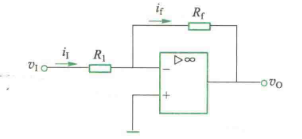
\includegraphics[width=0.7\linewidth]{image/3.png}
    \caption{反相比例放大器原理图}
    \label{fig:inverting-amplifier}
\end{figure}

由上式可以看出, 该电路的增益和运放的性能指标无关, 可以很方便地通过外围电阻的调节改变电路增益。

\begin{table}[h]
    \centering
    \caption{测试条件与结果}
    \begin{tabular}{cccccp{3.5cm}}
        \toprule
        测试条件 & \multicolumn{2}{c}{所选阻值} & 输出电压 & 放大倍数( 实测 ) & 输入输出波形\newline( 同一坐标下定量绘制 ) \\
        \cmidrule(lr){2-3} \cmidrule(lr){4-4} \cmidrule(lr){5-5}
        $v_i/V$ & $A$ & $R_i/\Omega$ \quad $R_f/\Omega$ & $v_o/V$ & $A$ & \\
        \midrule
        $2\cos(1000\pi t)$ & -3 &10K\quad 30K&5.88V&-2.94&\\
        \bottomrule
    \end{tabular}
\end{table}
\begin{figure}

    \centering
    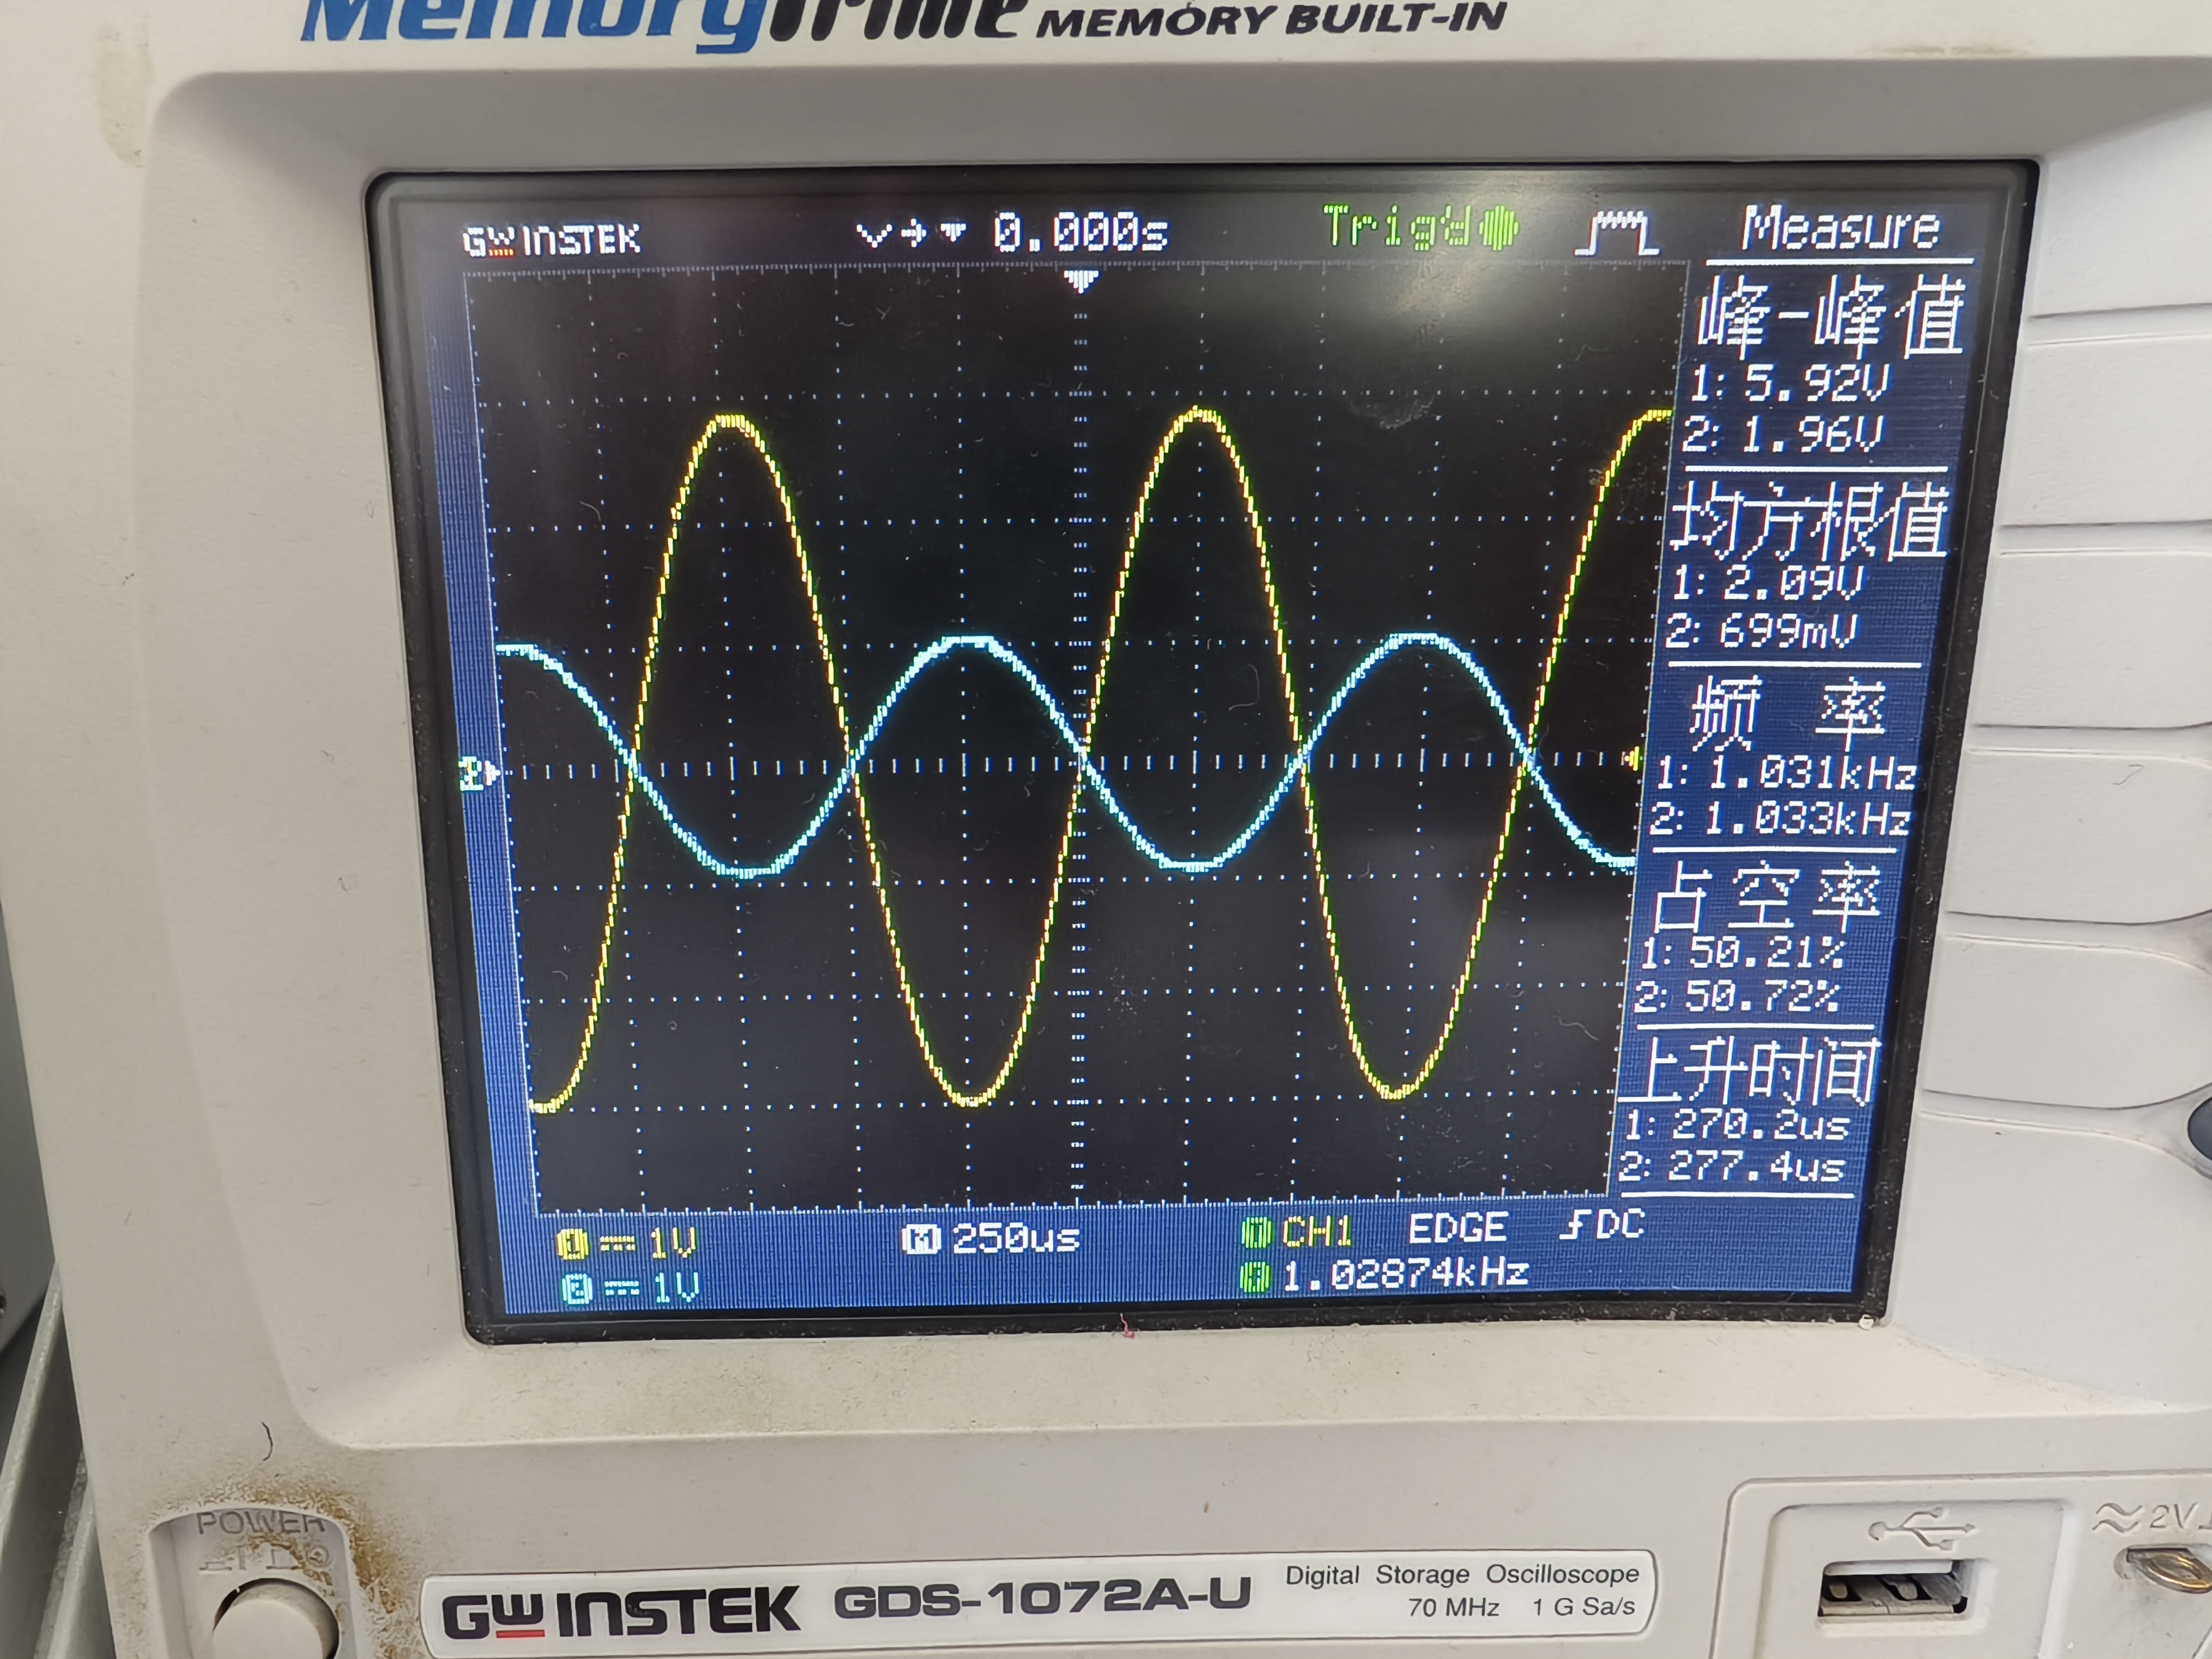
\includegraphics[width=0.7\linewidth]{image/5.jpg}
    \caption{反相比例放大器输入输出波形}
    \label{fig:inverting-amplifier-waveform}
\end{figure}

\clearpage
\subsubsection*{( 2 )同相比例放大器}

如图~\hyperref[fig:non-inverting-amplifier]{\ref{fig:non-inverting-amplifier}}是同相比例放大器原理图, 输入信号从同相端接入, 反相端通过电阻 $R_f$ 接地。同样依据两个基本原则“虚短”和“虚断”有

 $$
\begin{cases}
i_1 = i_f \\
v_- = v_+ = v_1
\end{cases}
$$ 
有

 $$
\frac{v_1}{R_1} = \frac{v_0 - v_1}{R_f}
$$ 

\begin{figure}[ht]
    \centering
    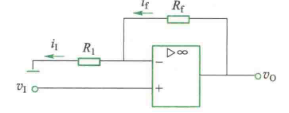
\includegraphics[width=0.7\linewidth]{image/4.png}
    \caption{同相比例放大器原理图}
    \label{fig:non-inverting-amplifier}
\end{figure}

\begin{table}[ht]
    \centering
    \caption{测试条件与结果}
    \begin{tabular}{cccccp{3.5cm}}
        \toprule
        测试条件 & \multicolumn{2}{c}{所选阻值} & 输出电压 & 放大倍数( 实测 ) & 输入输出波形( 同一坐标下定量绘制 ) \\
        \cmidrule(lr){2-3} \cmidrule(lr){4-4} \cmidrule(lr){5-5}
        $v_i/V$ & $A$ & $R_i/\Omega$ \quad $R_f/\Omega$ & $v_o/V$ & $A$& \\
        \midrule
        $2\cos(1000\pi t)$ & 2 &30K \quad 30K&3.04V&2&\\
        \bottomrule
    \end{tabular}
\end{table}
\begin{figure}[ht]
    \centering
    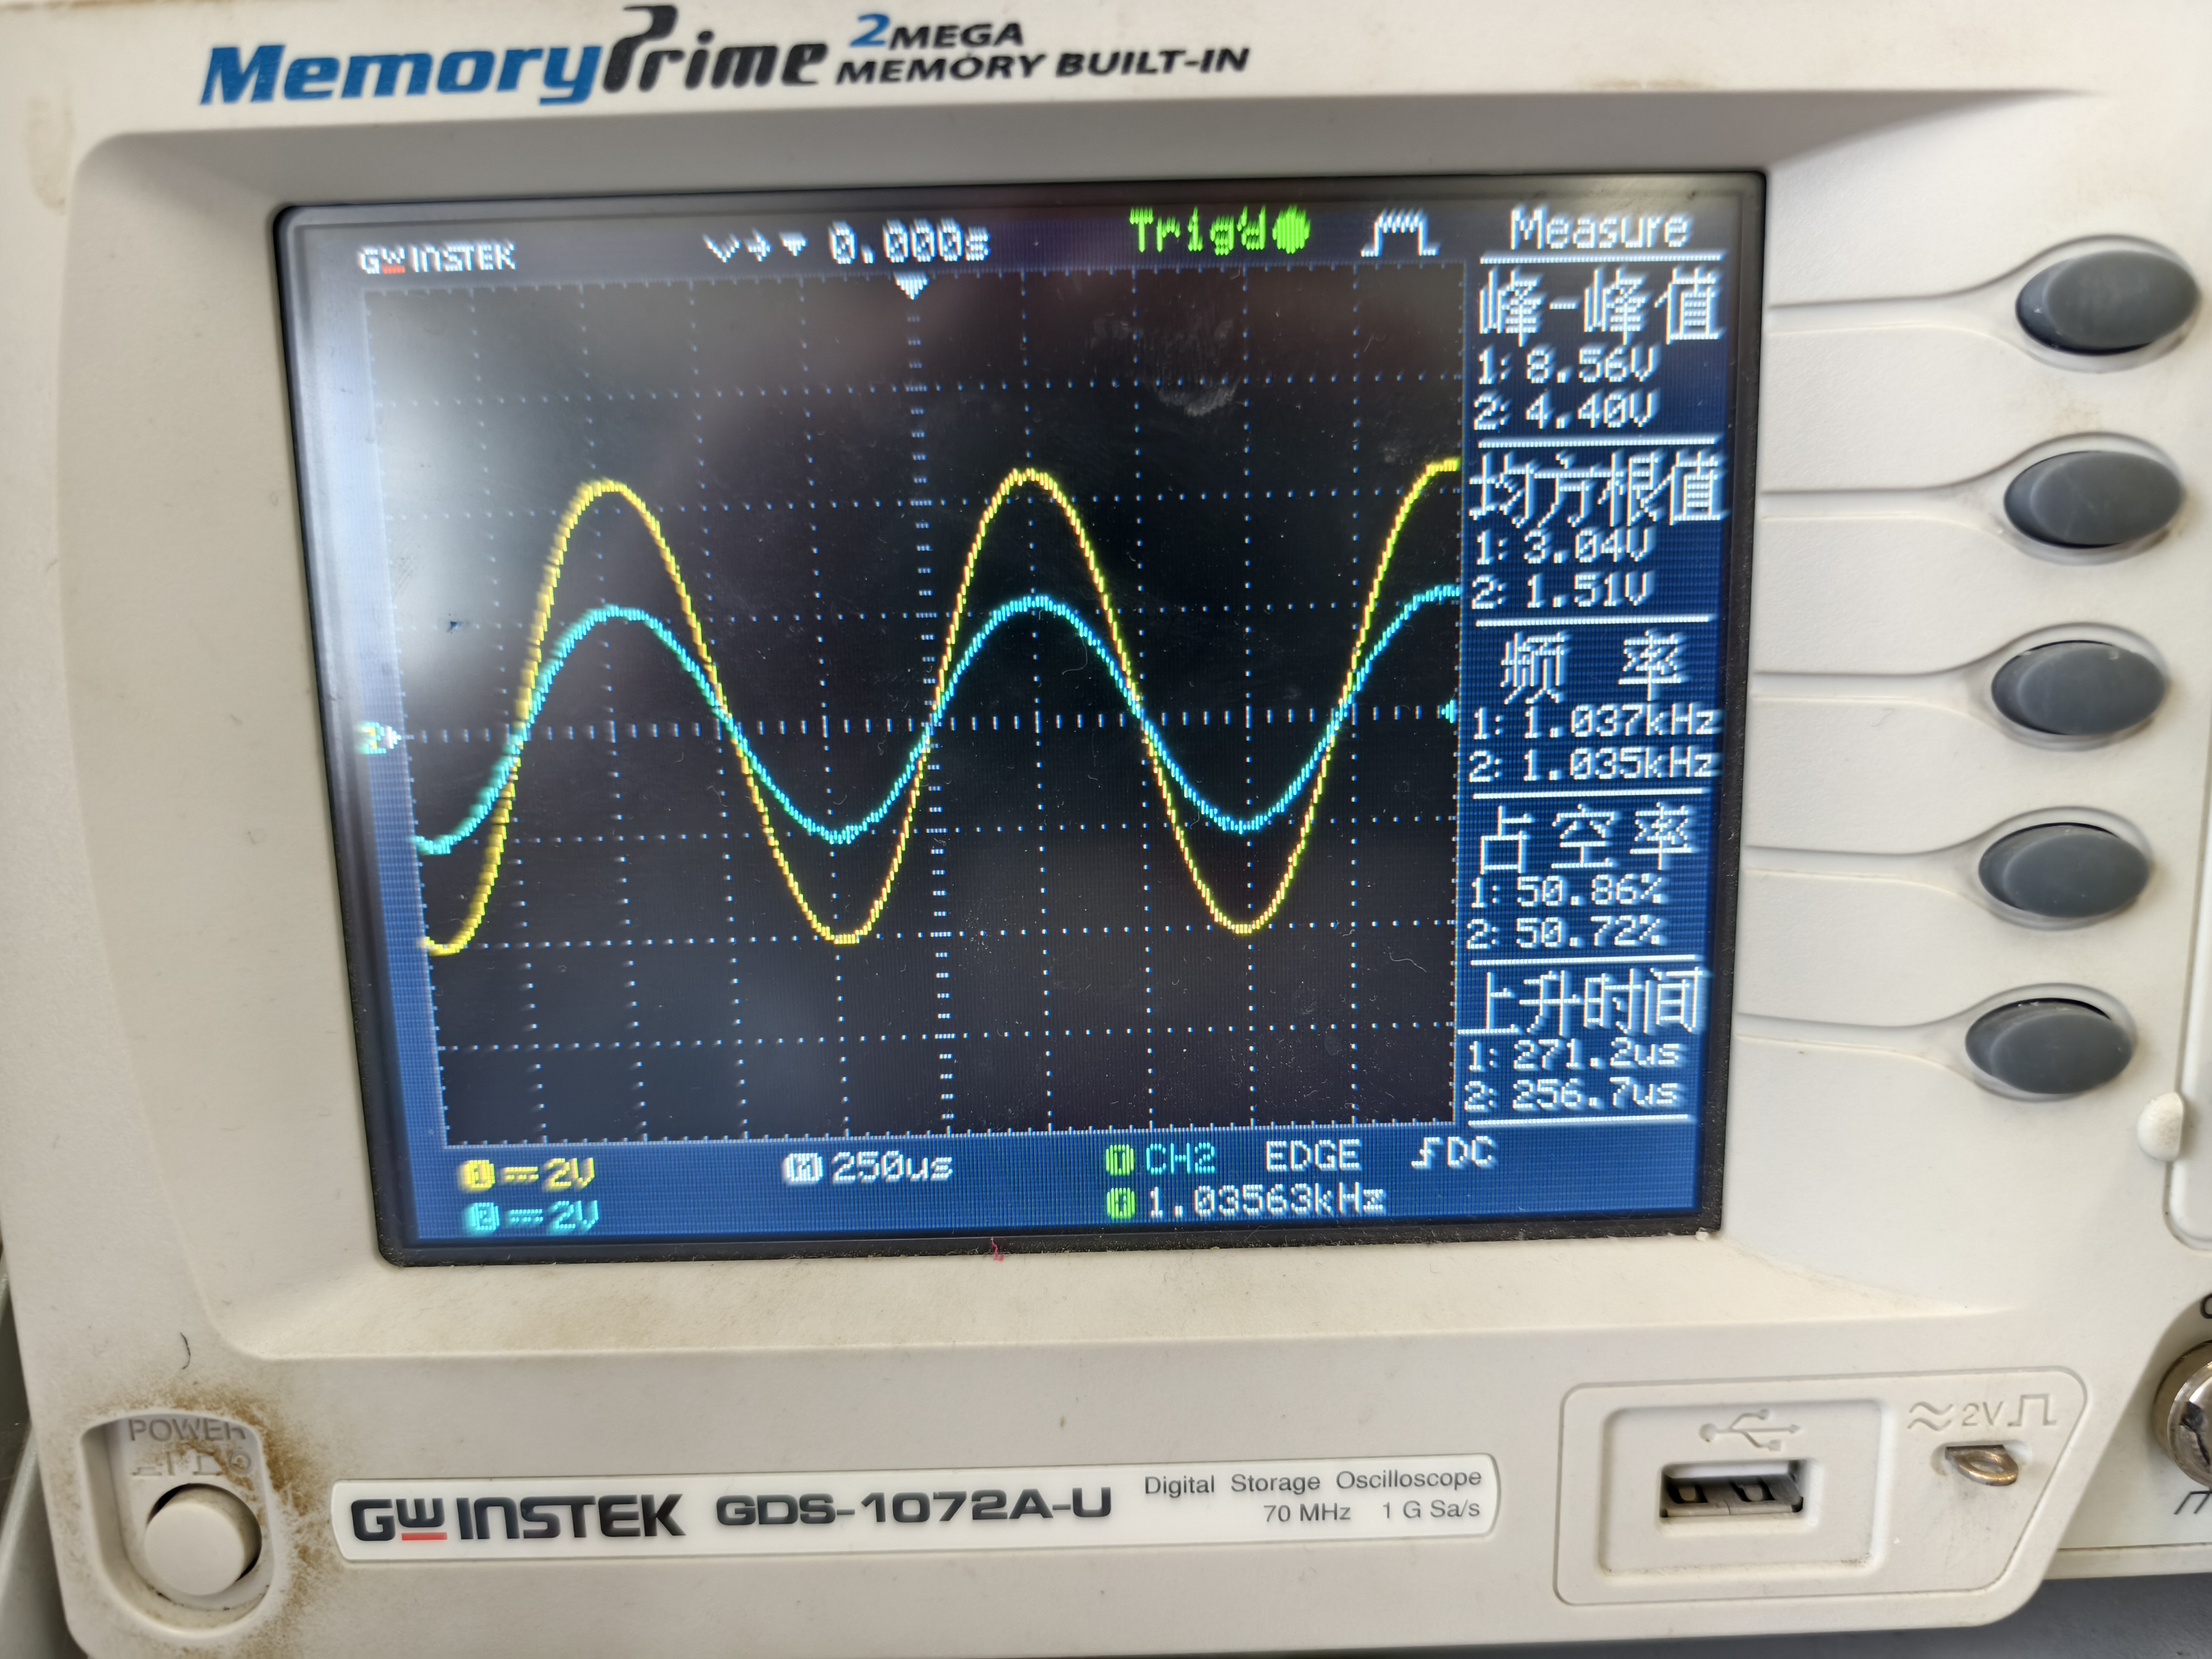
\includegraphics[width=0.7\linewidth]{image/6.jpg}
    \caption{同相比例放大器输入输出波形}
    \label{fig:non-inverting-amplifier-waveform}
\end{figure}

\newpage

\subsection{实验结论}
……
\section{思考题}
\subsection{题面}
\begin{enumerate}[leftmargin=50pt,label=(\arabic*)] % 设置序号格式为(1)
    \item 试分析同相比例放大器与反相比例放大器之间的优缺点
    \item 若要改变放大器的增益, 试问须调节电路中的哪些参数?


\end{enumerate}
\subsection{回答}

\begin{enumerate}[leftmargin=50pt,label=(\arabic*)] % 设置序号格式为(1)
    \item 同相放大器:同相放大器的最大的优点就是输入阻抗接近无穷大, 常常作为电压跟随器使用, 进行隔离。但其的最大缺点是输入没有“虚地”, 存在较大的共模电压, 抗干扰的能力较差, 使用时, 要求运放有较高的共模抑制比。
    
    反相放大器:反相放大器的最大的优点是输入端的正反相电位差接近为0, 只存在差模信号, 抗干扰能力强。但反相放大器的最大缺点是输入的阻抗很小, 等于信号输入端的串联电阻阻值。
    \item 主要有内部电路中放大级数、三极管或场效应管的增益、反馈强度等相关参数。
\end{enumerate}

\section{实验体会及建议}
\subsection{实验体会}
测量时应注意小心调试仪器, 尽量将读数稳定在误差允许范围内进行读数。
\subsection{建议}
注意电源正负极的接入, 防止反接造成仪器损坏, 注意正负电压的接入, 防止反接造成仪器损坏。

\end{document}
